%!TEX program = xelatex
\documentclass[a4paper,14pt]{extreport}

\usepackage{fontspec}
\setmainfont{Times New Roman}
\setmonofont{Courier New}
\setsansfont{Arial}

\usepackage[russian]{babel}

\usepackage[left=30mm, right=10mm, top=20mm, bottom=20mm]{geometry}
\usepackage{indentfirst}
\setlength{\parindent}{1.25cm}
\emergencystretch=3em

\usepackage{graphicx}
\graphicspath{{images/}}
\usepackage{float}

\usepackage{titlesec}
\usepackage{tocloft}
\usepackage{listings}
\usepackage{xcolor}
\usepackage{caption}
\usepackage{xurl}
\usepackage{hyperref}
\usepackage{amsmath, amssymb}
\usepackage{booktabs, tabularx, array}

\hypersetup{
    colorlinks=true,
    linkcolor=black,
    filecolor=black,
    urlcolor=blue,
    citecolor=black
}

% Настройка заголовков
\titleformat{\chapter}[block]
  {\filcenter\fontsize{16pt}{20pt}\selectfont\bfseries}
  {\ifnum\value{chapter}>0 Глава \thechapter.\quad\fi}
  {0pt}
  {}
\titlespacing*{\chapter}{0pt}{0pt}{18pt}

\titleformat{\section}[block]
  {\filcenter\fontsize{14pt}{17pt}\selectfont\bfseries}
  {\thesection\quad}
  {0pt}
  {}
\titlespacing*{\section}{0pt}{16pt}{10pt}

\renewcommand{\thesection}{\arabic{chapter}.\arabic{section}.}

% Настройка подписей к рисункам, таблицам и листингам
\captionsetup[figure]{labelsep=period, name=Рис., justification=centering}
\renewcommand{\thefigure}{%
  \ifnum\value{chapter}=0 1%
  \else\arabic{chapter}.\arabic{figure}%
  \fi
}

\captionsetup[table]{labelsep=period, name=Таблица, justification=raggedright, singlelinecheck=false}
\renewcommand{\thetable}{%
  \ifnum\value{chapter}=0 1%
  \else\arabic{chapter}.\arabic{table}%
  \fi
}

\renewcommand{\lstlistingname}{Листинг}
\AtBeginDocument{%
  \renewcommand{\thelstlisting}{\arabic{chapter}.\arabic{lstlisting}}%
}

% Настройка оглавления (Содержание)
\addto\captionsrussian{\renewcommand{\contentsname}{Содержание}}
\addto\captionsrussian{\renewcommand{\bibname}{Список использованных источников}}

\renewcommand{\cfttoctitlefont}{\hfill\fontsize{16pt}{20pt}\selectfont\bfseries}
\renewcommand{\cftaftertoctitle}{\hfill\null}
\setlength{\cftbeforetoctitleskip}{0pt}
\setlength{\cftaftertoctitleskip}{24pt}

\renewcommand{\cftchapfont}{\normalfont\bfseries}
\renewcommand{\cftchappagefont}{\normalfont\bfseries}
\renewcommand{\cftchapleader}{\hfill}
\renewcommand{\cftchappresnum}{Глава~}
\renewcommand{\cftchapaftersnum}{.}
\newlength{\mylen}
\settowidth{\mylen}{\bfseries Глава~1.\ }
\cftsetrmarg{25mm}
\setlength{\cftchapnumwidth}{\mylen}
\setlength{\cftbeforechapskip}{14pt}

\renewcommand{\cftsecfont}{\normalfont}
\renewcommand{\cftsecpagefont}{\normalfont}
\renewcommand{\cftsecleader}{\cftdotfill{\cftdotsep}}
\renewcommand{\cftsecaftersnum}{}
\setlength{\cftsecindent}{\mylen}
\setlength{\cftsecnumwidth}{12mm}
\setlength{\cftbeforesecskip}{4pt}

% Стиль листингов
\definecolor{codekeyword}{RGB}{236, 0, 139}   % #ec008b magenta
\definecolor{codestring}{RGB}{147, 0, 209}    % #9300d1 purple
\definecolor{codecomment}{RGB}{0, 153, 0}     % #009900 green
\definecolor{codenumbers}{RGB}{127, 127, 127} % #7f7f7f gray

\lstdefinelanguage{TypeScript}{
  keywords={abstract, any, as, async, await, boolean, break, case, catch, class, const, constructor, continue, debugger, default, delete, do, else, enum, export, extends, false, finally, for, from, function, get, if, implements, import, in, instanceof, interface, let, module, new, null, number, of, package, private, protected, public, readonly, return, set, static, string, super, switch, symbol, this, throw, true, try, type, typeof, var, void, while, with, yield},
  sensitive=true,
  comment=[l]{//},
  morecomment=[s]{/*}{*/},
  morestring=[b]',
  morestring=[b]",
  morestring=[b]`
}

\lstdefinestyle{courseworkstyle}{
    backgroundcolor=\color{white},
    basicstyle=\fontsize{9.5pt}{11.5pt}\selectfont\ttfamily,
    breakatwhitespace=false,
    breaklines=true,
    captionpos=b,
    keepspaces=true,
    numbers=left,
    numbersep=8pt,
    numberstyle=\fontsize{6pt}{8pt}\selectfont\color{codenumbers},
    showspaces=false,
    showstringspaces=false,
    showtabs=false,
    tabsize=2,
    frame=single,
    rulecolor=\color{black},
    keywordstyle=\color{codekeyword}\bfseries,
    commentstyle=\color{codecomment}\itshape,
    stringstyle=\color{codestring},
    aboveskip=8pt,
    belowskip=8pt,
    escapeinside={(*@}{@*)}
}
\lstset{style=courseworkstyle}

\begin{document}

% --- ТИТУЛЬНЫЙ ЛИСТ ---
\begin{titlepage}
\noindent
\begin{minipage}[c]{0.14\textwidth}
  
\includegraphics[width=\linewidth]{logo.png}
\end{minipage}%
\hfill
\begin{minipage}[c]{0.84\textwidth}
  \centering
  \fontsize{8pt}{9.5pt}\selectfont
  \textbf{МИНИСТЕРСТВО СЕЛЬСКОГО ХОЗЯЙСТВА РОССИЙСКОЙ ФЕДЕРАЦИИ}\\
  \vspace{1mm}
  ФЕДЕРАЛЬНОЕ ГОСУДАРСТВЕННОЕ БЮДЖЕТНОЕ ОБРАЗОВАТЕЛЬНОЕ УЧРЕЖДЕНИЕ ВЫСШЕГО ОБРАЗОВАНИЯ\\
  \vspace{1mm}
  \textbf{«РОССИЙСКИЙ ГОСУДАРСТВЕННЫЙ АГРАРНЫЙ УНИВЕРСИТЕТ -- МСХА имени К.~А.~ТИМИРЯЗЕВА»}\\
  \vspace{1mm}
  \textbf{(ФГБОУ ВО РГАУ -- МСХА имени К.~А.~Тимирязева)}
\end{minipage}

\vspace{3mm}
\hrule height 0.4pt
\vspace{1.5pt}
\hrule height 0.4pt

\vfill

\begin{center}
  \fontsize{12pt}{14pt}\selectfont
  Институт экономики и управления\\[1.5mm]
  Кафедра статистики и кибернетики\\[3.5mm]
  Направление: 09.03.02 Информационные системы и технологии\\[1.5mm]
  Направленность:\\[1mm]
  Системный анализ
\end{center}

\vfill

\begin{center}
  {\fontsize{20pt}{24pt}\selectfont\bfseries КУРСОВОЙ ПРОЕКТ\par}
  \vspace{3mm}
  {\fontsize{13pt}{16pt}\selectfont на тему: «Проектирование и разработка многопользовательской блог-платформы с интеллектуальным помощником»\par}
\end{center}

\vfill

\hfill
\begin{minipage}{0.52\textwidth}
  \fontsize{12pt}{14.5pt}\selectfont
  Выполнила:\\[1mm]
  Студентка 3 курса группы Д-Э317\\[1mm]
  Преснякова Вероника Борисовна\\[3mm]
  Дата регистрации КП\\
  на кафедре: \underline{\hspace{38mm}}\\[3.5mm]
  Допущен к защите\\[1mm]
  Руководитель:\\[2mm]
  \underline{\hspace{72mm}}\\
  \vspace{-2.5mm}
  {\fontsize{8.5pt}{10pt}\selectfont\hspace*{12mm} учёная степень, учёное звание, ФИО\par}\vspace{3mm}
  Члены комиссии:\\[2mm]
  \underline{\hspace{47mm}}\;\underline{\hspace{20mm}}\\
  \vspace{-2.5mm}
  {\fontsize{8.5pt}{10pt}\selectfont учёная степень, учёное звание, ФИО\hfill подпись\hspace*{2mm}\par}\vspace{2mm}
  \underline{\hspace{47mm}}\;\underline{\hspace{20mm}}\\
  \vspace{-2.5mm}
  {\fontsize{8.5pt}{10pt}\selectfont учёная степень, учёное звание, ФИО\hfill подпись\hspace*{2mm}\par}\vspace{3mm}
  Оценка \underline{\hspace{51mm}}\\[2.5mm]
  Дата защиты \underline{\hspace{43mm}}
\end{minipage}

\vfill

\begin{center}
  \fontsize{14pt}{17pt}\selectfont
  Москва 2026
\end{center}
\end{titlepage}

% Сброс номера страницы
\setcounter{page}{2}

% --- СОДЕРЖАНИЕ ---
\tableofcontents
\newpage

% --- ВВЕДЕНИЕ ---
\chapter*{Введение}
\addcontentsline{toc}{chapter}{Введение}

В современных условиях экспоненциального роста объемов цифровой информации и возрастающей когнитивной нагрузки эффективное управление персональными знаниями становится критически важным фактором личной и профессиональной продуктивности. Ведение регулярных структурированных заметок позволяет пользователям фиксировать идеи, формировать базы знаний и снижать уровень информационной тревожности. Однако традиционные инструменты управления заметками и блог-платформы сталкиваются с фундаментальной проблемой долгосрочного удержания (retention): большинство пользователей забрасывают регулярное ведение записей уже в первые недели использования из-за отсутствия мгновенной обратной связи, однообразия рутинного процесса и необходимости постоянного волевого усилия.

Современные исследования в области проектирования пользовательского опыта показывают, что сухая самодисциплина значительно уступает механизмам эмоциональной вовлеченности и фоновой геймификации. Внедрение виртуального питомца, состояние и показатели благополучия которого органично зависят от регулярности и качества ведения заметок, формирует устойчивый паттерн возврата в приложение. При этом критически важно, чтобы игровые элементы функционировали в «теневом» режиме, не отвлекая пользователя всплывающими окнами и визуальным шумом в процессе интеллектуальной работы с текстом.

Дополнительным фактором, определяющим эффективность современной платформы управления контентом, является наличие интеллектуального помощника. По мере роста объема накопленных материалов ручная категоризация становится трудоемкой, а поиск информации затрудняется. Применение алгоритмов семантического автотегирования и кластеризации позволяет автоматизировать систематизацию базы знаний, преобразуя хаотичный набор заметок в упорядоченную структуру.

Создание высоконагруженных многопользовательских систем такого типа предъявляет повышенные требования к архитектурной надежности, масштабируемости и сквозной типизации данных. Необходимость параллельной обработки пользовательских HTTP-запросов и тяжелых фоновых расчетов игровой экономики (пересчета уровней, агрегации опыта, начисления наград) требует бескомпромиссного разделения ответственности между компонентами, эффективного управления конкурентным доступом на уровне СУБД и модульной структуры клиентского кода.

\textbf{Актуальность темы} обусловлена необходимостью разработки производительной, надежной и масштабируемой блог-платформы для ведения заметок, сочетающей строгий инструмент для работы с контентом, адаптивную модель фоновой геймификации для повышения мотивации пользователей и интеллектуального помощника для автоматической смысловой обработки данных.

\textbf{Целью курсового проекта} является проектирование и разработка многопользовательской блог-платформы (веб-приложения заметок «PigKeep») с интеллектуальным помощником и виртуальным питомцем, обладающей высокой степенью отказоустойчивости, строгой сквозной типизацией и оптимизированной архитектурой данных.

Для достижения поставленной цели необходимо решить следующие \textbf{задачи}:
\begin{enumerate}
  \item Исследовать теоретические основы построения многоуровневых клиент-серверных архитектур, паттернов проектирования (SoC, Repository Pattern, Event Log) и методологии Feature-Sliced Design (FSD) для модульной организации фронтенда.
  \item Провести сравнительный анализ и обосновать выбор современного технологического стека, обеспечивающего сквозную типобезопасность (TypeScript, PostgreSQL 18, Drizzle ORM, Express 5, React 19, Vite, TanStack Query, Zustand, Zod, Tailwind CSS).
  \item Разработать математическую модель игровой экономики приложения на основе аппарата многомерной взвешенной средней (расчет Индекса удовольствия, шкалы HP и системы коэффициентов опыта XP) и концепцию интеллектуального помощника.
  \item Спроектировать реляционную схему базы данных в третьей нормальной форме (3NF), разработать структуру связей, составные покрывающие индексы и механизмы полнотекстового поиска с ранжированием релевантности.
  \item Реализовать серверную часть (валидацию на уровне middleware, агрегацию прогресса с помощью обобщенных табличных выражений CTE, транзакционные рекомендательные блокировки \texttt{pg\_\allowbreak advisory\_\allowbreak xact\_\allowbreak lock}) и клиентский интерфейс с поддержкой оптимистичных обновлений.
  \item Разработать комплексную стратегию тестирования по паттерну AAA (модульные, интеграционные и контрактные тесты с изоляцией состояния) и реализовать процесс безопасного развертывания системы в контейнерах Docker.
\end{enumerate}

\textbf{Объектом исследования} выступают веб-приложения для управления персональными заметками и блог-платформы, интегрированные с механизмами игровой экономики и интеллектуальной поддержки пользователей.

\textbf{Предметом исследования} являются программно-архитектурные решения, структуры данных реляционной СУБД, алгоритмы вычисления многомерных показателей продуктивности и механизмы синхронизации состояния клиент-серверной системы.

\textbf{Научная новизна} работы заключается в синтезе метода многомерной взвешенной средней с архитектурным паттерном Event Log и транзакционными рекомендательными блокировками PostgreSQL, что позволило реализовать неинтрузивную фоновую игровую модель, гарантирующую консистентность состояния и защиту от состояний гонки без снижения пропускной способности системы.

\textbf{Практическая значимость} результатов заключается в создании полнофункционального веб-приложения PigKeep, обладающего готовым к развертыванию контейнеризированным монорепозиторием, компонентной базой на основе методологии FSD, оптимизированным ядром базы данных и набором автоматизированных тестов, обеспечивающих высокую надежность и удобство дальнейшего масштабирования продукта.

\textbf{Структура работы}: курсовой проект состоит из введения, двух глав, заключения и списка использованных источников.

\newpage

% --- ГЛАВА 1 ---
\chapter{ТЕОРЕТИЧЕСКИЕ ОСНОВЫ И АРХИТЕКТУРНЫЕ ПАТТЕРНЫ ВЕБ-ПРИЛОЖЕНИЙ}

\section{Архитектурные паттерны и организация приложения}

Современная инженерия программного обеспечения, особенно в контексте высоконагруженных клиент-серверных систем, требует бескомпромиссного соблюдения принципа разделения ответственности (Separation of Concerns, SoC). Монолитные структуры, в которых логика обработки сетевых запросов тесно переплетена с бизнес-правилами и SQL-запросами, неизбежно приводят к деградации кодовой базы (так называемому «спагетти-коду») и невозможности эффективного масштабирования. В основе серверной части проекта лежит строгая многоуровневая архитектура (Layered Architecture), которая обеспечивает жесткую изоляцию компонентов системы в зависимости от их семантической роли~\cite{ref1}.

В рамках платформы Node.js жизненный цикл любого HTTP-запроса проходит через строго детерминированную цепочку уровней абстракции. Изначально запрос попадает в маршрутизатор (Router), задача которого сводится исключительно к определению конечной точки. Далее запрос проходит через слой промежуточных обработчиков (Middleware), где осуществляется авторизация и валидация полезной нагрузки. После этого управление передается контроллеру, выступающему в роли оркестратора бизнес-процессов. Однако контроллер не взаимодействует с базой данных напрямую; для абстрагирования слоя персистентности применяется классический паттерн «Репозиторий» (Repository Pattern)~\cite{ref1}.

Паттерн «Репозиторий» выступает в качестве посредника между логикой предметной области и уровнем сопоставления данных, используя интерфейсы, аналогичные коллекциям объектов~\cite{ref4}. Применение репозиториев позволяет скрыть сложность построения SQL-запросов и детали реализации конкретной системы управления базами данных (СУБД) от бизнес-логики. Это архитектурное решение не только повышает читаемость кода, но и является критически важным для стратегии тестирования. Благодаря инверсии зависимостей (Dependency Inversion), реальный репозиторий, обращающийся к PostgreSQL, может быть легко заменен на mock-объект в модульных тестах, что позволяет проверять бизнес-логику в абсолютной изоляции от внешнего ввода-вывода~\cite{ref5}.

\begin{lstlisting}[language=TypeScript, caption={Определение интерфейса репозитория заметок и контроллера}, label={lst:repository-pattern}]
interface RepositoryType {
  repo: {
    getNotesFromDB: (params?: {
      search?: string | undefined
      tagId?: string | undefined
      isArchive?: boolean | undefined
      isDeleted?: boolean | undefined
    }) => Promise<Note[]>
    getNoteByIdFromDB: (noteId: string) => Promise<Note | undefined>
    createNoteFromDB: (noteData: NoteCreateIn) => Promise<Note | undefined>
    putNoteFromDB: (noteId: string, noteData: NotePutIn) => Promise<Note | undefined>
    patchNoteFromDB: (noteId: string, noteData: NotePatchIn) => Promise<Note | undefined>
    deleteNoteFromDB: (noteId: string) => Promise<number | null>
    getNoteTagsFromDB: (noteId: string) => Promise<{ id: string; name: string }[]>
    addTagToNoteInDB: (noteId: string, tagId: string) => Promise<{ note_id: string; tag_id: string }[]>
    removeTagFromNoteInDB: (noteId: string, tagId: string) => Promise<number | null>
  }
}

export function controller({ repo }: RepositoryType) {
  const {
    getNotesFromDB,
    getNoteByIdFromDB,
    createNoteFromDB,
    putNoteFromDB,
    patchNoteFromDB,
    deleteNoteFromDB,
    getNoteTagsFromDB,
    addTagToNoteInDB,
    removeTagFromNoteInDB,
  } = repo;
}
\end{lstlisting}

На клиентской стороне сложность управления состоянием, компонентами и их взаимосвязями диктует необходимость использования продвинутых методологий организации кодовой базы. Традиционный подход группировки файлов по их техническому типу (папки \texttt{components}, \texttt{hooks}, \texttt{services}) быстро теряет свою эффективность по мере роста проекта, так как не отражает бизнес-домен приложения~\cite{ref6}. В связи с этим для фронтенда была выбрана архитектурная методология Feature-Sliced Design (FSD)~\cite{ref1}. В отличие от классических подходов, FSD группирует код на основе логики предметной области, решая фундаментальную проблему запутанных зависимостей~\cite{ref8}.

Методология Feature-Sliced Design вводит строгую иерархию слоев (Layers), направленную от глобального к локальному:
\begin{itemize}
  \item \textbf{App}: Слой инициализации приложения. Здесь располагаются корневые настройки, глобальные стили, базовые провайдеры контекста и конфигурация маршрутизации~\cite{ref8}.
  \item \textbf{Pages}: Слой страниц. Модули этого слоя собирают полноценные пользовательские экраны путем композиции сущностей, фич и виджетов~\cite{ref9}.
  \item \textbf{Widgets}: Самостоятельные, крупные композиционные блоки интерфейса, такие как панель навигации или сложный дашборд управления питомцем~\cite{ref9}.
  \item \textbf{Features}: Слой пользовательских сценариев, несущих конкретную бизнес-ценность (например, функционал «создать заметку», «покормить питомца», «добавить тег»). Фичи инкапсулируют логику взаимодействия пользователя с системой~\cite{ref9}.
  \item \textbf{Entities}: Слой бизнес-сущностей. Содержит интерфейсы данных, UI-карточки и логику, напрямую связанную с объектами предметной области (пользователь, заметка, питомец), но без привязки к конкретным действиям~\cite{ref9}.
  \item \textbf{Shared}: Слой переиспользуемых инфраструктурных модулей. Включает базовые UI-компоненты (кнопки, инпуты), утилиты, конфигурации API-клиентов и абстракции, не зависящие от бизнес-логики~\cite{ref10}.
\end{itemize}

Краеугольным камнем FSD является правило однонаправленного потока зависимостей: модуль имеет право импортировать только те модули, которые располагаются на строго нижестоящих слоях~\cite{ref10}. Это архитектурное ограничение гарантирует, что изменения в высокоуровневых компонентах (например, на страницах) никогда не приведут к каскадным поломкам в базовых сущностях. Кроме того, FSD внедряет концепцию Public API: каждый модуль (слайс) экспортирует свою функциональность исключительно через единый файл \texttt{index.ts}. Все внутренние файлы модуля остаются инкапсулированными и недоступными для прямого импорта извне, что защищает систему от неконтролируемого связывания (tight coupling)~\cite{ref7}. На рисунке~\ref{fig:fsd-layers} приведена иерархия слоев FSD.

\begin{figure}[H]
  \centering
  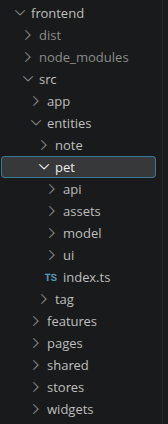
\includegraphics[width=0.40\textwidth]{fsd_layers.png}
  \caption{Иерархия слоев методологии Feature-Sliced Design}
  \label{fig:fsd-layers}
\end{figure}

Геймификационная составляющая сервиса, отвечающая за развитие питомца, опирается на архитектурный паттерн Event Log, который идеологически близок к концепции Event Sourcing. В традиционных системах CRUD любое действие пользователя (например, создание заметки) привело бы к мгновенному изменению состояния питомца (увеличению опыта в таблице \texttt{pets}). Однако такой подход уязвим для состояний гонки и затрудняет аудит~\cite{ref1}. Вместо мутации состояния, паттерн Event Log фиксирует действия пользователя как серию атомарных, неизменяемых событий в специализированной таблице. Эти факты в дальнейшем асинхронно обрабатываются фоновым планировщиком с использованием транзакционных рекомендательных блокировок (Advisory Locks), что позволяет реализовать сложную математическую логику без блокировки основного потока выполнения пользовательских запросов.

\newpage

\section{Обоснование технологического стека}

Выбор технологического стека является одним из наиболее критичных этапов проектирования, поскольку он определяет пределы масштабируемости, производительности и надежности системы. В проекте стек технологий продиктован строгими требованиями к сквозной типизации данных (End-to-End Type Safety) и отказоустойчивости~\cite{ref1}.

В качестве системы управления реляционными базами данных выбрана PostgreSQL 18~\cite{ref1}. Выбор в пользу PostgreSQL, в противовес легковесной синхронной SQLite или документо-ориентированной MongoDB, обусловлен несколькими архитектурными преимуществами. Во-первых, природа данных (заметки, теги, связи между ними) носит ярко выраженный реляционный характер, требующий соблюдения ограничений внешних ключей (Foreign Key Constraints). Во-вторых, PostgreSQL реализует архитектуру Multi-Version Concurrency Control (MVCC) --- многоверсионное управление конкурентным доступом~\cite{ref12}.

В традиционных СУБД читающие транзакции блокируют пишущие, и наоборот. MVCC элегантно решает эту проблему: каждая транзакция работает с собственным консистентным «снимком» (snapshot) данных на момент своего начала~\cite{ref12}. Технически это реализуется за счет скрытых системных колонок \texttt{xmin} (идентификатор транзакции, создавшей версию строки) и \texttt{xmax} (идентификатор транзакции, удалившей или обновившей строку)~\cite{ref12}. Благодаря этому, длительные фоновые расчеты опыта питомца могут выполняться без ущерба для пользователей, которые в этот же момент интенсивно создают или читают свои заметки. PostgreSQL также предоставляет мощнейшие инструменты полнотекстового поиска на уровне ядра СУБД, что критически важно для приложения заметок.

Для интеграции серверной логики с СУБД выбран инструмент Drizzle ORM~\cite{ref1}. В экосистеме TypeScript исторически доминировал инструмент Prisma, однако в контексте архитектуры данного проекта Drizzle ORM предоставляет неоспоримые преимущества. Prisma использует парадигму «Schema-first»: разработчик описывает структуру базы данных в специализированном файле \texttt{.prisma}, после чего запускает процесс кодогенерации, который создает типизированный клиент~\cite{ref16}. Несмотря на удобство абстракции, Prisma исторически опиралась на тяжеловесный runtime-движок (Query Engine), что приводило к значительному расходу оперативной памяти и проблемам с задержками при «холодном старте» (cold start) в serverless/edge окружениях~\cite{ref17}.

Drizzle ORM, напротив, исповедует принцип «SQL-first» и «Codebase-first». Описание схемы базы данных выполняется на языке TypeScript~\cite{ref16}. Отсутствие этапа кодогенерации означает, что типы выводятся мгновенно в процессе написания кода (Type Inference). Главное преимущество Drizzle --- нулевые накладные расходы на runtime. Drizzle напрямую транслирует вызовы функций в оптимизированные SQL-строки без промежуточного слоя движка, что сокращает накладные расходы на формирование запроса до $\sim 0.5$~мс~\cite{ref17}. Подробное сравнение подходов приведено в таблице~\ref{tab:orm-comparison}.

\begin{table}[H]
  \caption{Сравнительный анализ Drizzle ORM и Prisma ORM}
  \label{tab:orm-comparison}
  \vspace{2mm}
  \centering
  \small
  \begin{tabularx}{\textwidth}{|>{\raggedright\arraybackslash}p{4.2cm}|>{\raggedright\arraybackslash}X|>{\raggedright\arraybackslash}X|}
    \hline
    \textbf{Архитектурный аспект} & \textbf{Drizzle ORM} & \textbf{Prisma ORM} \\
    \hline
    Парадигма проектирования & SQL-first, Codebase-first~\cite{ref16} & Schema-first, абстракция объектов~\cite{ref16} \\
    \hline
    Накладные расходы (Overhead) & Минимальные, прямая генерация SQL-строк~\cite{ref17} & Наличие Query Compiler (WASM в Prisma 7)~\cite{ref17} \\
    \hline
    Система типизации & Мгновенный вывод (Inference) без кодогенерации~\cite{ref16} & Строгая типизация через \texttt{prisma generate}~\cite{ref16} \\
    \hline
    Выполнение в Edge (Serverless) & Нативная поддержка, нулевые зависимости~\cite{ref16} & Улучшено в v7, но требует дополнительных адаптеров~\cite{ref17} \\
    \hline
    Подход к миграциям & Прозрачные, редактируемые SQL-файлы~\cite{ref16} & Скрыты за абстрактным DSL~\cite{ref16} \\
    \hline
  \end{tabularx}
\end{table}

В листинге~\ref{lst:drizzle-schema} представлен фрагмент описания сущностей \texttt{pets}, \texttt{notes} и \texttt{tags} с использованием синтаксиса Drizzle ORM.

\begin{lstlisting}[language=TypeScript, caption={Описание схемы сущностей pets, notes и tags в Drizzle ORM}, label={lst:drizzle-schema}]
export const pets = pgTable('pets', {
  id: uuid('id')
    .primaryKey()
    .default(sql`gen_random_uuid()`),
  name: varchar('name', { length: 255 }).notNull(),
  level: integer('level').default(1).notNull(),
  progress: integer('progress').default(0).notNull(),
  pleasureIndex: integer('pleasure_index').default(100).notNull(),
})

export const notesTable = pgTable('notes', {
  id: uuid('id')
    .primaryKey()
    .default(sql`gen_random_uuid()`),
  user_id: uuid()
    .default(sql`gen_random_uuid()`)
    .notNull(),
  title: text().default('').notNull(),
  content: text().default('').notNull(),
  isArchive: boolean().default(false),
  isDeleted: boolean().default(false),
})

export const tagsTable = pgTable('tags', {
  id: uuid('id')
    .primaryKey()
    .default(sql`gen_random_uuid()`),
  name: text().notNull(),
})
\end{lstlisting}

Серверная инфраструктура базируется на платформе Node.js и веб-фреймворке Express 5. Использование Node.js позволяет унифицировать язык программирования (TypeScript) на всем стеке, обеспечивая возможность переиспользования интерфейсов данных между клиентом и сервером. Express 5 привносит нативную поддержку асинхронных операций (Promises) в обработчиках маршрутов, избавляя разработчиков от необходимости оборачивать каждый контроллер в громоздкие блоки \texttt{try/catch} или использовать сторонние библиотеки вроде \texttt{express-async-handler}~\cite{ref1}.

На стороне клиентского приложения архитектура состояния разделена на две независимые области. Фреймворк React 19 в связке со сборщиком Vite обеспечивает компонентную модель и феноменально быструю горячую замену модулей (HMR). Для управления серверным состоянием (Server State) --- данными, которые асинхронно извлекаются из API и требуют кэширования, дедупликации запросов и фоновой синхронизации --- внедрена библиотека TanStack Query v5~\cite{ref1}. Управление локальным пользовательским состоянием, таким как состояние модальных окон, тема оформления или временные фильтры, делегировано библиотеке Zustand. В отличие от React Context или Redux, Zustand предоставляет минималистичный API, основанный на хуках, и точечно обновляет компоненты, предотвращая избыточный рендеринг всего дерева~\cite{ref1}.

Сквозная валидация данных реализуется с помощью библиотеки Zod, позволяющей единожды описать схему данных и использовать ее как для валидации на сервере, так и для форм на клиенте. Визуальная составляющая формируется посредством Tailwind CSS v4, который, используя utility-first подход, радикально уменьшает объем генерируемого CSS-кода за счет атомарных классов~\cite{ref1}.

\newpage

% --- ГЛАВА 2 ---
\chapter{ПРОЕКТИРОВАНИЕ И ПРОГРАММНАЯ РЕАЛИЗАЦИЯ СИСТЕМЫ}

\section{Математическая модель игровой экономики и интеллектуальный помощник}

Сердцем платформы, отличающим его от конкурентов, является сложная математическая модель игровой экономики. Основная бизнес-цель данной модели --- создание устойчивого паттерна возврата (retention) и долгосрочного удержания пользователя через психологию привязанности к виртуальному питомцу~\cite{ref1}.

Центральной метрикой системы является Индекс удовольствия (Health/\allowbreak Happiness Points, HP), неформально именуемый «Свинометром». Для вычисления этого индекса применяется алгоритм многомерной средней. Модель не просто суммирует количество написанных символов, а оценивает комплексную полезность действий пользователя через систему весов. В расчет берутся такие векторы, как регулярность входов в приложение (streak), объем и структурированность заметок, а также частота использования тегов (полезная организация информации).

Математический расчет осуществляется в несколько этапов. Сначала каждый $j$-й показатель активности пользователя $x_j$ за отчетные сутки нормируется относительно установленного целевого эталона (дневной нормы) $X_j^{\text{norm}}$:
\begin{equation}
  z_j = \min\left(1, \frac{x_j}{X_j^{\text{norm}}}\right),
  \label{eq:norm}
\end{equation}
где $x_j$ --- фактическое число действий $j$-го типа за расчетный период; $X_j^{\text{norm}}$ --- эталонная суточная норма активности; $z_j \in [0; 1]$ --- коэффициент выполнения нормы.

Интегральный синтетический показатель настроения и благополучия питомца вычисляется по формуле многомерной взвешенной средней:
\begin{equation}
  \bar{I} = 100 \times \frac{\sum_{j=1}^{m} w_j \cdot z_j}{\sum_{j=1}^{m} w_j},
  \label{eq:index}
\end{equation}
где $m$ --- количество учитываемых типов активности ($m = 4$); $w_j$ --- весовые коэффициенты значимости действий. При создании новой заметки вес составляет $w_1 = 20$ (норма $X_1^{\text{norm}} = 3$); при категоризации тегами $w_2 = 15$ (норма $X_2^{\text{norm}} = 4$); при редактировании и обновлении $w_3 = 10$ (норма $X_3^{\text{norm}} = 5$); при ежедневном входе в приложение $w_4 = 5$ (норма $X_4^{\text{norm}} = 1$). Полученный суточный индекс $\bar{I} \in [0; 100]$ определяет шкалу здоровья и настроения питомца.

Полученный индекс HP выступает в роли динамического множителя для накопления опыта (XP). Накопление опыта позволяет питомцу визуально эволюционировать. Если индекс HP находится на высоком уровне (что свидетельствует об активном и качественном ведении заметок), к получаемому базовому опыту применяется стимулирующий коэффициент $\times 1.2$. В случае длительного бездействия пользователя алгоритм фиксирует падение Индекса удовольствия, что приводит к активации штрафного коэффициента $\times 0.5$. Подобная механика создает эффект FOMO (Fear Of Missing Out --- страх упущенной выгоды). Для предотвращения злоупотреблений и намеренного флуда бессмысленными записями в систему внедрен жесткий лимит --- пользователь не может получить более 500 XP за одни календарные сутки~\cite{ref1}.

Для практической реализации заявленной темы курсового проекта в архитектуру сервиса закладывается интеллектуальный помощник (AI Smart Assistant). Ассистент персонифицирован в лице питомца Бориса и выполняет следующие задачи:
\begin{enumerate}
  \item \textbf{Семантическое автотегирование в реальном времени}: в момент сохранения заметки фоновый алгоритм анализирует текст заголовка и тела, извлекая ключевые тематические сущности и предлагая 2--3 наиболее релевантных тега в один клик.
  \item \textbf{Смысловая кластеризация заметок}: периодический анализ векторных представлений (эмбеддингов) текстов неструктурированных заметок выявляет скрытые тематические группы и предлагает объединить разрозненные мысли в единую категорию.
  \item \textbf{Геймифицированная интеграция}: принятие рекомендаций интеллектуального помощника рассматривается системой как операция структурирования данных, поощряя пользователя дополнительным приростом опыта и повышением Индекса удовольствия питомца.
\end{enumerate}

\section{Проектирование реляционной схемы базы данных}

Проектирование реляционной схемы базы данных выполнено в строгом соответствии с правилами третьей нормальной формы (3NF). Это архитектурное решение исключает дублирование данных и защищает систему от аномалий модификации (update anomalies). Основные сущности системы образуют следующую структуру:
\begin{itemize}
  \item Таблица \texttt{notes} (заметки). Содержит первичный ключ (UUID), заголовок, текстовое содержимое и временные метки создания/изменения.
  \item Таблица \texttt{tags} (теги). Инкапсулирует название тега.
  \item Таблица \texttt{noteTags} (связывающая таблица). Необходима для физической реализации связи «многие ко многим», позволяя одной заметке иметь множество тегов, а одному тегу относиться к множеству заметок.
  \item Таблица \texttt{action\_logs}. Является реализацией паттерна Event Log, храня иммутабельные записи о каждом действии пользователя для последующего асинхронного начисления XP~\cite{ref1}.
\end{itemize}

В листинге~\ref{lst:notetags-schema} представлена программная реализация связующей таблицы и отношений многие-ко-многим с использованием Drizzle ORM.

\begin{lstlisting}[language=TypeScript, caption={Реализация связи многие-ко-многим между заметками и тегами в Drizzle ORM}, label={lst:notetags-schema}]
export const noteTagsTable = pgTable(
  'noteTags',
  {
    note_id: uuid('note_id')
      .notNull()
      .references(() => notesTable.id, { onDelete: 'cascade' }),
    tag_id: uuid('tag_id')
      .notNull()
      .references(() => tagsTable.id, { onDelete: 'cascade' }),
  },
  (table) => [primaryKey({ columns: [table.tag_id, table.note_id] })]
)

export const noteTagsRelations = defineRelations({ tagsTable, notesTable, noteTagsTable }, (r) => ({
  tagsTable: {
    notesTable: r.many.notesTable({
      from: r.tagsTable.id.through(r.noteTagsTable.tag_id),
      to: r.notesTable.id.through(r.noteTagsTable.note_id),
    }),
  },
  notesTable: {
    tagsTable: r.many.tagsTable({
      from: r.notesTable.id.through(r.noteTagsTable.note_id),
      to: r.tagsTable.id.through(r.noteTagsTable.tag_id),
    }),
  },
}))
\end{lstlisting}

В листинге~\ref{lst:action-logs-schema} приведено описание таблицы журнала действий \texttt{action\_\allowbreak logs} и ее индексов.

\begin{lstlisting}[language=TypeScript, caption={Описание таблицы журнала событий action\_logs и индексов}, label={lst:action-logs-schema}]
export const actionLogs = pgTable(
  'action_logs',
  {
    id: uuid('id')
      .primaryKey()
      .default(sql`gen_random_uuid()`),
    petId: uuid('pet_id')
      .notNull()
      .references(() => pets.id, { onDelete: 'cascade' }),
    actionTypeId: integer('action_type_id')
      .notNull()
      .references(() => actionTypes.id, { onDelete: 'restrict' }),
    createdAt: timestamp('created_at', { withTimezone: true })
      .defaultNow()
      .notNull(),
  },
  (table) => [
    index('action_logs_pet_id_idx').on(table.petId),
    index('action_logs_created_at_idx').on(table.createdAt),
    index('idx_action_logs_cron_covering').on(
      table.createdAt,
      table.petId,
      table.actionTypeId
    ),
  ]
)
\end{lstlisting}

Для обеспечения мгновенного поиска по накопленной базе знаний приложение не использует стандартный оператор LIKE, который крайне неэффективен при поиске по большим объемам текста из-за невозможности использования B-Tree индексов при поиске по подстроке. Вместо этого задействован встроенный механизм полнотекстового поиска PostgreSQL. Текстовые данные преобразуются с помощью функции \texttt{to\_tsvector} в оптимизированный вектор лексем (с удалением стоп-слов и приведением к корню слова). Поисковые запросы пользователя обрабатываются через \texttt{to\_tsquery}. Использование функции \texttt{ts\_rank} позволяет базе данных самостоятельно ранжировать возвращаемые результаты на основе плотности и расположения искомых слов в заметке, обеспечивая высокую релевантность выдачи~\cite{ref1}.

Производительность фоновых задач (например, ежедневного пересчета агрегированного прогресса) критически зависит от индексов. В базе данных спроектированы составные покрывающие индексы. Они сконструированы таким образом, что содержат не только ключи для фильтрации (например, \texttt{user\_id}, \texttt{created\_at}), но и сами агрегируемые значения. Это позволяет планировщику PostgreSQL выполнять запросы в режиме Index-Only Scan. В этом режиме данные извлекаются исключительно из структуры индекса, расположенной в оперативной памяти, без необходимости ресурсоемкого чтения основных страниц таблицы (heap) с диска, что обеспечивает масштабируемость системы~\cite{ref1}.

\section{Программная реализация серверной и клиентской логики}

Практическая реализация серверной логики фокусируется на обеспечении отказоустойчивости и глубокой защите (Defense in Depth). Централизованная валидация данных реализована с использованием паттерна Middleware. Любой входящий HTTP-запрос (например, создание заметки) перехватывается промежуточным слоем, где его полезная нагрузка (body) сопоставляется со строгими схемами, описанными на базе Zod. Если данные не соответствуют контракту (например, отсутствует заголовок или текст превышает допустимый лимит), Middleware мгновенно прерывает дальнейшую обработку и возвращает клиенту HTTP статус 400 (Bad Request). Это гарантирует, что в контроллеры и репозитории попадают исключительно очищенные и корректные данные, предотвращая инъекции и сбои в бизнес-логике~\cite{ref1}.

Одной из самых сложных алгоритмических задач в бэкенде является реализация функции \texttt{processDailyPetProgress}. Поскольку расчет дневного прогресса зависит от сотен записей в таблице \texttt{action\_logs}, построчное извлечение и обновление каждой записи на уровне Node.js неизбежно привело бы к проблеме N+1 запросов и переполнению пула соединений. Для оптимизации этой задачи используются Common Table Expressions (CTE) --- обобщенные табличные выражения, реализуемые через оператор WITH в SQL. Использование CTE позволяет базе данных предварительно агрегировать события и вычислить итоговые инкременты опыта, а затем обновить таблицу питомцев одним атомарным запросом (Bulk Update) на уровне ядра СУБД~\cite{ref1}. В листинге~\ref{lst:recalc-query} представлен соответствующий фрагмент SQL-запроса с CTE.

\begin{lstlisting}[language=TypeScript, caption={Агрегация опыта и пересчет уровня питомца с использованием CTE}, label={lst:recalc-query}]
const recalculationQuery = sql<{
  id: string
  old_level: number
  new_level: number
  new_progress: number
}>`
  WITH daily_xp AS (
    SELECT
      ${actionLogs.petId} AS pet_id,
      SUM(${actionTypes.weight})::int AS earned_xp
    FROM ${actionLogs}
    INNER JOIN ${actionTypes}
      ON ${actionLogs.actionTypeId} = ${actionTypes.id}
    WHERE
      ${actionLogs.createdAt} >= ${startDate}
      AND ${actionLogs.createdAt} < ${endDate}
    GROUP BY ${actionLogs.petId}
  )
  UPDATE ${pets} AS p
  SET
    level = CASE
      WHEN lr.required_xp IS NOT NULL
           AND (p.progress + dxp.earned_xp) >= lr.required_xp
        THEN p.level + 1
      ELSE p.level
    END,
    progress = CASE
      WHEN lr.required_xp IS NOT NULL
           AND (p.progress + dxp.earned_xp) >= lr.required_xp
        THEN (p.progress + dxp.earned_xp) - lr.required_xp
      ELSE p.progress + dxp.earned_xp
    END
  FROM daily_xp dxp
  LEFT JOIN ${levelRequirements} lr
    ON lr.level = p.level
  WHERE p.id = dxp.pet_id
  RETURNING
    p.id,
    (p.level - CASE
      WHEN lr.required_xp IS NOT NULL AND (p.progress + dxp.earned_xp) >= lr.required_xp THEN 1
      ELSE 0
    END) AS old_level,
    p.level AS new_level,
    p.progress AS new_progress;
`
\end{lstlisting}

Интерфейс пользователя спроектирован с учетом высоких требований к отзывчивости (UX). Для нивелирования сетевых задержек реализован паттерн оптимистичных обновлений средствами TanStack Query v5~\cite{ref1}. При добавлении тега или заметки интерфейс не дожидается ответа от сервера (HTTP 201 Created). В функции \texttt{onMutate} система делает «снимок» (snapshot) текущего состояния кэша, после чего мгновенно обновляет локальные данные, перерисовывая интерфейс с нулевой задержкой~\cite{ref19}. Фоном запрос отправляется на сервер. Если сервер возвращает ошибку (например, потеря соединения), срабатывает механизм отката (rollback) в блоке \texttt{onError}, который восстанавливает состояние интерфейса до ранее сохраненного снимка. Контроль форм и их реактивность осуществляются библиотекой \texttt{react-hook-form}, которая бесшовно интегрирована с Zod-схемами~\cite{ref1}.

На рисунке~\ref{fig:dashboard} представлен интерфейс главного дашборда приложения PigKeep, объединяющий сетку заметок и панель виртуального питомца.

\begin{figure}[H]
  \centering
  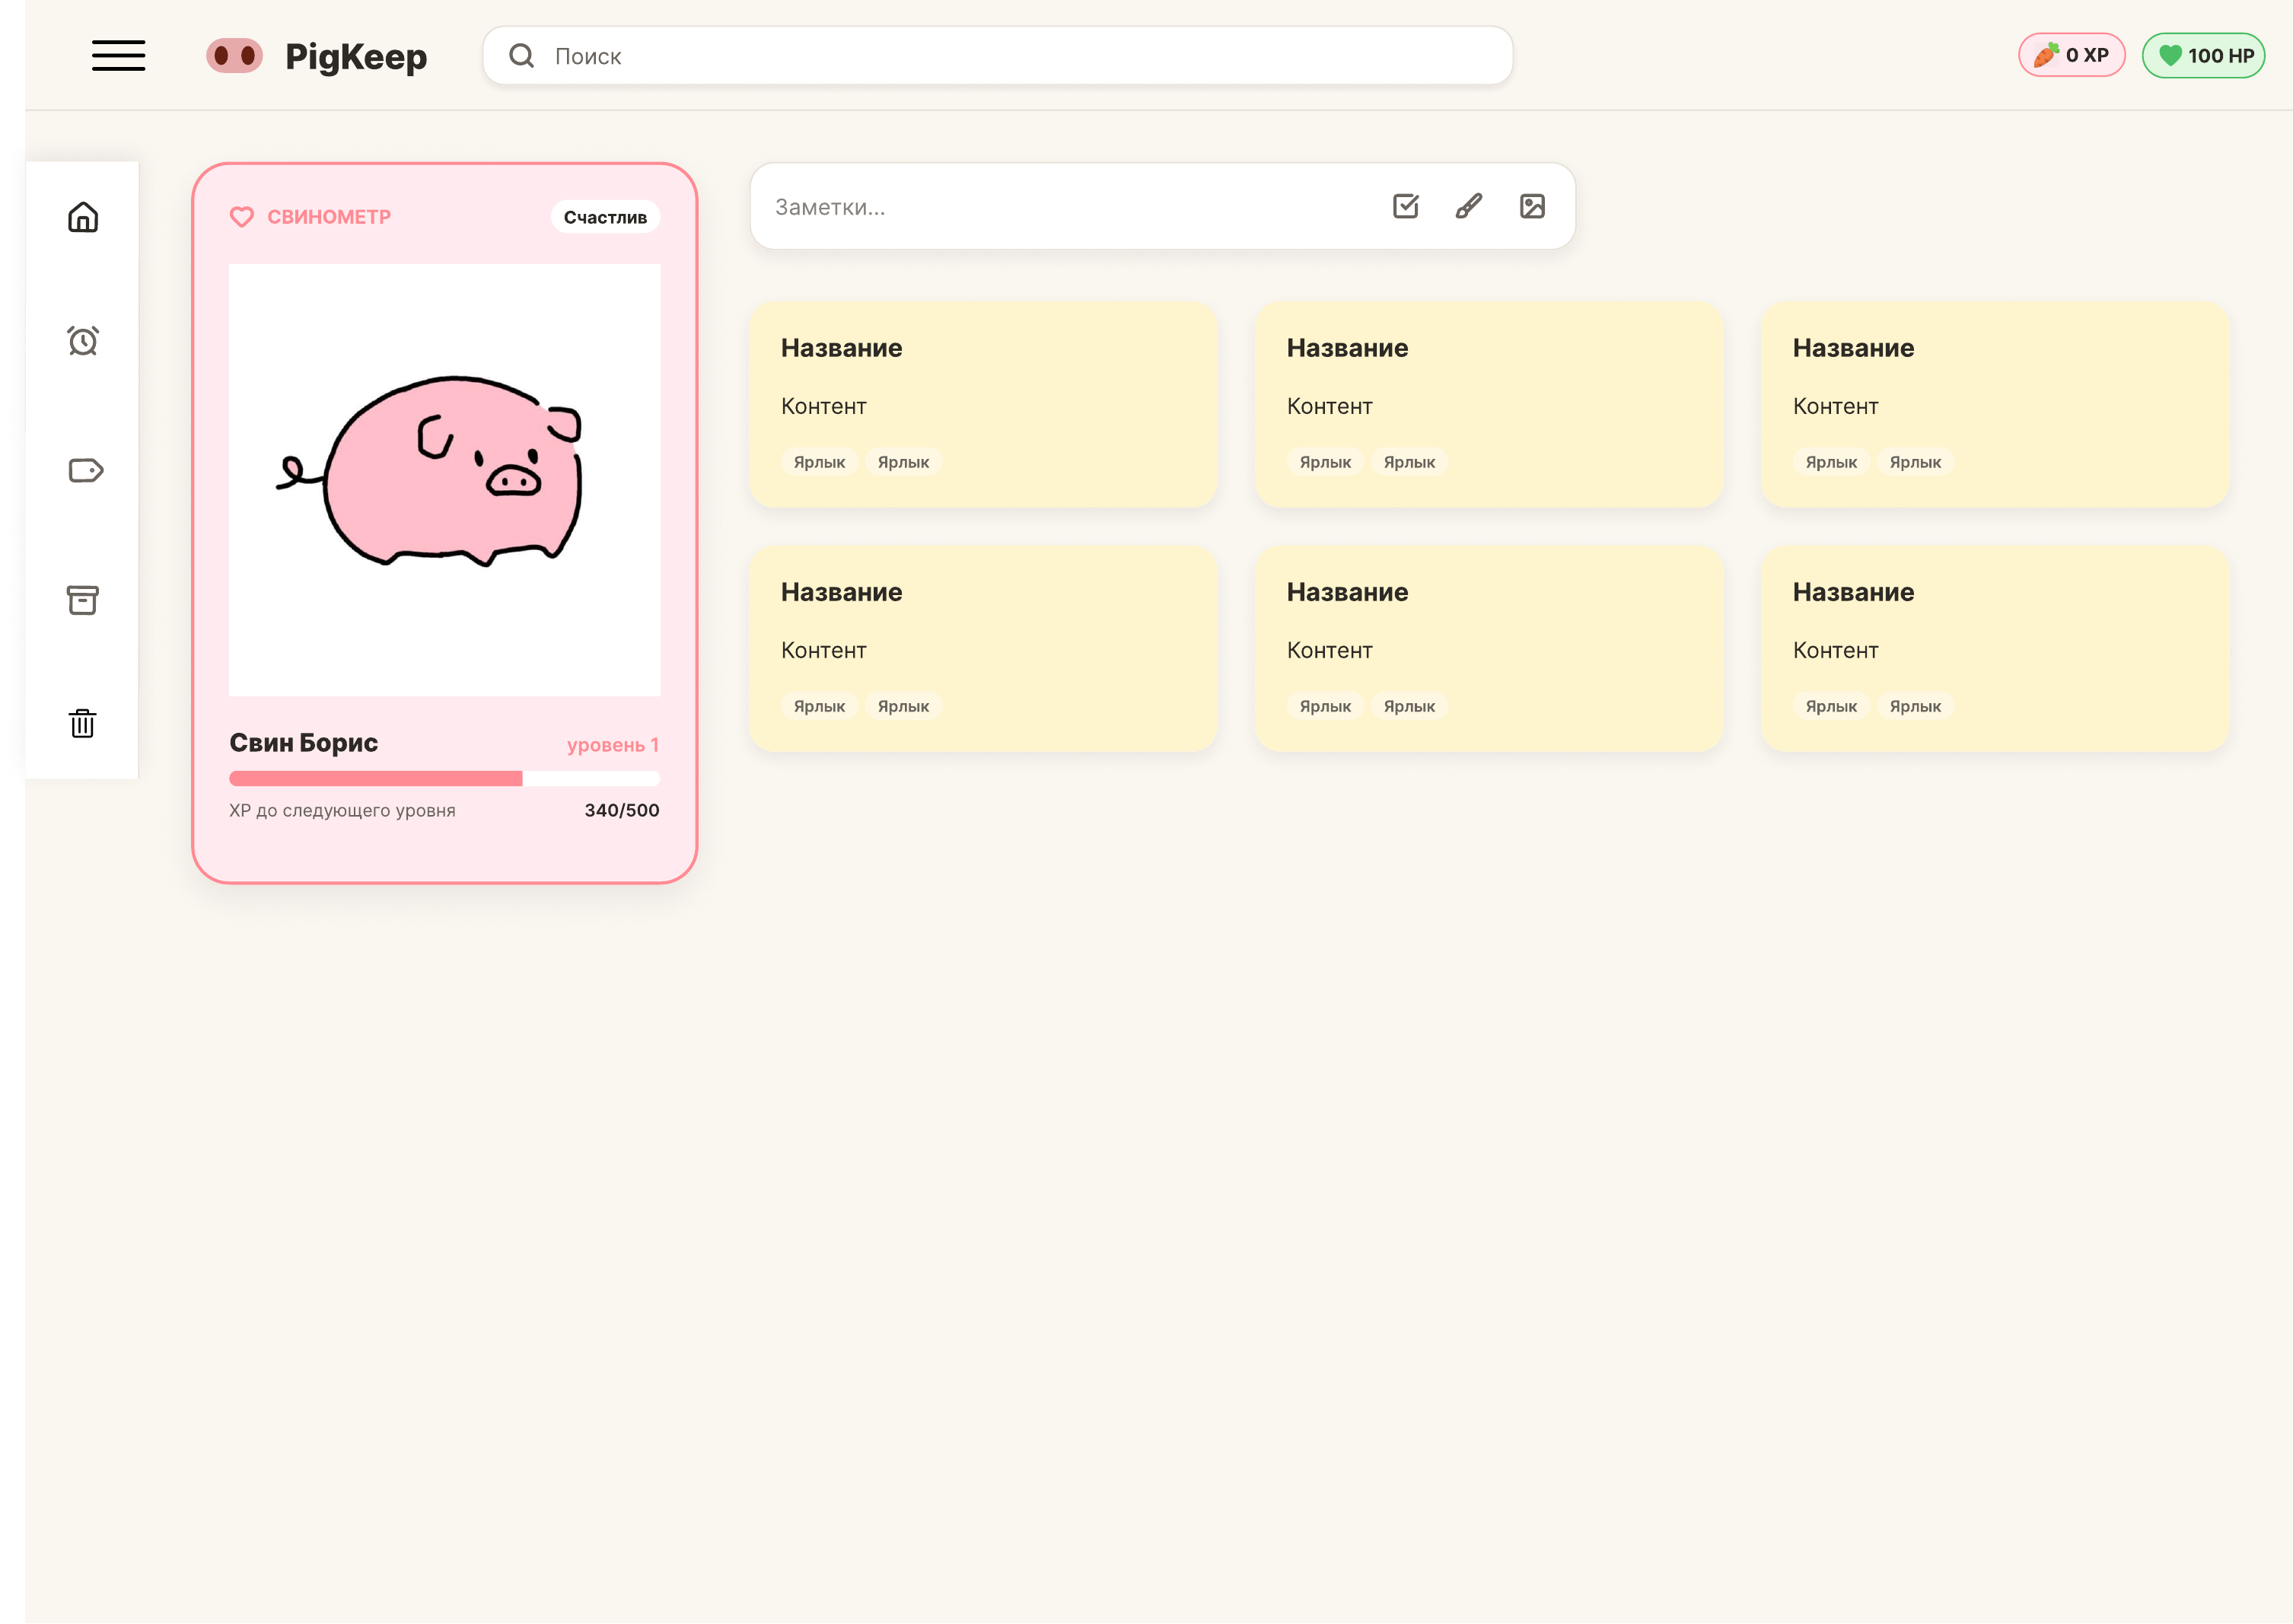
\includegraphics[width=0.88\textwidth]{dashboard-1.png}
  \caption{Интерфейс главного экрана веб-приложения PigKeep}
  \label{fig:dashboard}
\end{figure}

\section{Обеспечение безопасности и параллельного выполнения}

Безопасность параллельного выполнения фоновых задач обеспечивается через транзакционные рекомендательные блокировки (Advisory Locks) PostgreSQL. Если система развернута в нескольких экземплярах (например, в Kubernetes), существует риск, что несколько контейнеров попытаются выполнить ежедневный пересчет одновременно, что приведет к дублированию начисления опыта~\cite{ref11}. Использование блокировок строк (SELECT ... FOR UPDATE) в данном случае не подходит, так как физические строки могут еще не существовать~\cite{ref18}. PostgreSQL предоставляет функцию \texttt{pg\_advisory\_xact\_lock}, которая создает логическую блокировку на основе сгенерированного приложением 64-битного ключа~\cite{ref1}. В отличие от блокировок уровня сессии (\texttt{pg\_advisory\_lock}), транзакционные блокировки (\texttt{pg\_advisory\_xact\_lock}) автоматически освобождаются при коммите или откате транзакции. Это исключает риск «зависших» блокировок, особенно при использовании пулеров соединений, таких как PgBouncer, где понятие сессии размыто~\cite{ref11}.

Процесс развертывания системы стандартизирован посредством контейнеризации в Docker с применением Multi-stage сборок (многоэтапных сборок). Этот подход решает две задачи: минимизацию размера образа и повышение безопасности. На первом этапе (Builder) в контейнер устанавливаются все зависимости (включая devDependencies), выполняется проверка типов TypeScript и сборка React-приложения через Vite. На втором этапе создается чистый, легковесный образ на базе Nginx. В него копируются только скомпилированные артефакты из папки dist. Важнейшим аспектом безопасности является использование образа nginx-unprivileged, который запускает веб-сервер от имени ограниченного пользователя (не root). Благодаря такому подходу итоговый размер Docker-образа фронтенда составляет всего 26.5 МБ~\cite{ref1}.

В листинге~\ref{lst:dockerfile-backend} приведен многоэтапный Dockerfile для сборки и развертывания серверной части приложения.

\begin{lstlisting}[language=bash, caption={Многоэтапный Dockerfile для серверной части приложения}, label={lst:dockerfile-backend}]
FROM node:24.21.0-bookworm-slim AS builder
WORKDIR /usr/src/app
COPY package*.json ./
COPY backend/package*.json ./backend/
COPY packages/shared/package*.json ./packages/shared/
RUN npm ci
COPY packages/shared ./packages/shared
COPY backend ./backend
WORKDIR /usr/src/app/backend
RUN npm run build:prod

FROM node:24.21.0-bookworm-slim AS runner
WORKDIR /usr/src/app
COPY package*.json ./
COPY backend/package*.json ./backend/
COPY packages/shared/package*.json ./packages/shared/
RUN npm ci --omit=dev
COPY --from=builder /usr/src/app/packages/shared ./packages/shared
COPY --from=builder /usr/src/app/backend/build ./backend/build
COPY --from=builder /usr/src/app/backend/migrations ./migrations
EXPOSE 3000
USER node
CMD [ "node", "backend/build/server.js"]
\end{lstlisting}

В листинге~\ref{lst:dockerfile-frontend} приведен Dockerfile для развертывания клиентской части с сервером Nginx от имени непривилегированного пользователя.

\begin{lstlisting}[language=bash, caption={Многоэтапный Dockerfile для развертывания клиентской части}, label={lst:dockerfile-frontend}]
FROM node:24.21.0-bookworm-slim AS builder
WORKDIR /usr/src/app
COPY package*.json ./
COPY frontend/package*.json ./frontend/
COPY packages/shared/package*.json ./packages/shared/
RUN npm ci
COPY packages/shared ./packages/shared
COPY frontend ./frontend
WORKDIR /usr/src/app/frontend
RUN npm run build

FROM nginxinc/nginx-unprivileged:alpine AS runner
COPY frontend/nginx.conf /etc/nginx/conf.d/default.conf
COPY --from=builder /usr/src/app/frontend/dist /usr/share/nginx/html
EXPOSE 8080
USER nginx
CMD ["nginx", "-g", "daemon off;"]
\end{lstlisting}

\section{Стратегия тестирования и контроль качества}

Обеспечение качества программного обеспечения базируется на комплексном тестировании. Модульное тестирование алгоритмов (таких как расчет Свинометра) и схем валидации выполняется в среде Vitest, которая обладает нативной поддержкой конфигураций Vite. Для проверки интеграции UI и логики запросов без развертывания реальной базы данных применяется Mock Service Worker (MSW). MSW перехватывает сетевые запросы на уровне Service Worker в браузере или Node.js, позволяя возвращать заранее подготовленные мок-ответы. Это дает возможность эффективно тестировать краевые случаи, например, гарантированно вызывать ошибки сервера (HTTP 500) для проверки корректности работы механизма оптимистичного отката в UI~\cite{ref1}.

В проекте реализована комплексная пирамида тестирования, охватывающая как клиентскую, так и серверную части, с фокусом на проверке реального поведения системы. На уровне контрактов (Vitest, Zod) проверяются граничные условия без запуска сервера. Интеграционное тестирование бэкенда (Supertest, Drizzle ORM, PostgreSQL) проверяет сквозное прохождение HTTP-запросов, работу полнотекстового поиска и соответствие БД нормальным формам.

В листинге~\ref{lst:test-pets-api} представлен интеграционный тест эндпоинта инициализации питомца с использованием библиотеки Supertest.

\begin{lstlisting}[language=TypeScript, caption={Интеграционный тест эндпоинта API питомца с использованием Supertest}, label={lst:test-pets-api}]
describe('GET /api/v1/pets', () => {
  it('should auto-initialize and return default pet when no pet exists', async () => {
    const res = await request(app).get(BASE_URL)

    expect(res.status).toBe(200)
    expect(res.body.pet).toBeDefined()
    expect(res.body.pet).toMatchObject({
      name: 'Борис',
      level: 1,
      progress: 0,
      pleasureIndex: 100,
      requiredXp: 500,
      mood: 'happy',
    })
    expect(res.body.pet.id).toBeDefined()
  })
})
\end{lstlisting}

В листинге~\ref{lst:test-db-schemas} представлен модульный тест проверки колонок схемы базы данных на соответствие требованиям 3NF.

\begin{lstlisting}[language=TypeScript, caption={Тестирование колонок схемы базы данных}, label={lst:test-db-schemas}]
describe('Database Schemas (3NF)', () => {
  it('should define pets table with correct columns', () => {
    expect(pets.id).toBeDefined()
    expect(pets.name).toBeDefined()
    expect(pets.level).toBeDefined()
    expect(pets.progress).toBeDefined()
    expect(pets.pleasureIndex).toBeDefined()
  })
})
\end{lstlisting}

На фронтенде интеграционное тестирование (React Testing Library, MSW) оценивает реальные пользовательские сценарии, состояния загрузки и обработку ошибок интерфейса. Юнит-тестирование хуков гарантирует корректную инвалидацию кэша (TanStack Query) и управление таймерами, что предотвращает утечки памяти при размонтировании компонентов. В листинге~\ref{lst:test-petcard} приведен тест компонента отображения карточки питомца \texttt{PetCard}.

\begin{lstlisting}[language=TypeScript, caption={Тестирование компонента PetCard с использованием React Testing Library}, label={lst:test-petcard}]
describe('PetCard', () => {
  const mockPet: Pet = {
    id: 'pet-123',
    name: 'Борис',
    level: 2,
    progress: 340,
    requiredXp: 500,
    pleasureIndex: 90,
    mood: 'happy',
  }

  it("should render pet name with 'Свин' prefix, level, and XP progress", () => {
    renderWithProviders(<PetCard pet={mockPet} />)

    expect(screen.getAllByText('Свин Борис').length).toBeGreaterThan(0)
    expect(screen.getAllByText('уровень 2').length).toBeGreaterThan(0)
    expect(screen.getByText('340/500')).toBeInTheDocument()
    expect(screen.getByText('ХР до следующего уровня')).toBeInTheDocument()
  })
})
\end{lstlisting}

Тесты строятся по паттерну AAA (Arrange-Act-Assert) и используют вспомогательные хелперы для подготовки данных, исключая дублирование кода. Изоляция тестов достигается за счет полной очистки выделенной БД перед каждым запуском, применения независимых клиентов для кэша и оборачивания компонентов в кастомные провайдеры контекста (листинг~\ref{lst:test-isolation}).

\begin{lstlisting}[language=TypeScript, caption={Изоляция тестовых наборов через очистку таблиц базы данных}, label={lst:test-isolation}]
beforeEach(async () => {
  await test_db.execute(sql`TRUNCATE TABLE ${notesTable} CASCADE`)
})
\end{lstlisting}

\newpage

% --- ЗАКЛЮЧЕНИЕ ---
\chapter*{Заключение}
\addcontentsline{toc}{chapter}{Заключение}

В ходе выполнения курсового проекта была спроектирована и разработана многопользовательская блог-платформа (веб-приложение заметок «PigKeep») с интеллектуальным помощником и виртуальным питомцем, ориентированная на решение проблемы долгосрочного удержания пользователей и стимулирование регулярной продуктивной работы.

В процессе выполнения работы были достигнуты следующие ключевые результаты:
\begin{enumerate}
  \item Проведен углубленный анализ архитектурных паттернов организации современных распределенных веб-систем. Серверная часть реализована на основе многоуровневой архитектуры (Layered Architecture) с разделением слоев Router, Middleware, Controller и Repository. На клиенте применена архитектурная методология Feature-Sliced Design (FSD), что исключило неконтролируемые циклические зависимости и обеспечило изоляцию функциональных модулей (App, Pages, Widgets, Features, Entities, Shared).
  \item Обоснован и внедрен технологический стек, гарантирующий сквозную типобезопасность (End-to-End Type Safety): платформа Node.js, веб-фреймворк Express 5, клиентская библиотека React 19 в связке с Vite, инструментарий управления серверным состоянием TanStack Query v5, легковесный менеджер локального состояния Zustand, валидатор схем Zod и утилитарный фреймворк Tailwind CSS v4.
  \item В качестве системы персистентности выбрана СУБД PostgreSQL 18 и библиотека Drizzle ORM. Применение SQL-first подхода обеспечило нулевые runtime-издержки ($\sim 0.5$~мс на формирование запроса) и автоматический вывод TypeScript-типов без этапа кодогенерации, показав существенные преимущества перед Prisma ORM.
  \item Разработана и математически обоснована модель игровой экономики на базе аппарата многомерной взвешенной средней (Индекс удовольствия, или Свинометр). Алгоритм оценивает разнородные векторы пользовательской активности (регулярность сессий, создание и редактирование заметок, структурирование тегами), формируя динамические множители опыта ($\times 1.2$ и $\times 0.5$) и суточный лимит 500 XP для защиты от накрутки.
  \item Спроектирована реляционная схема базы данных в третьей нормальной форме (3NF), исключающая аномалии обновления. Внедрены составные покрывающие индексы, обеспечивающие выполнение аналитических выборок в режиме Index-Only Scan, а также механизм полнотекстового поиска PostgreSQL с векторизацией лексем и ранжированием релевантности.
  \item Разработана система асинхронного пересчета прогресса на базе Common Table Expressions (CTE), что устранило проблему $N+1$ запросов и обеспечило атомарный Bulk Update на уровне ядра СУБД. Конкурентная безопасность параллельных фоновых процессов гарантирована транзакционными рекомендательными блокировками \texttt{pg\_\allowbreak advisory\_\allowbreak xact\_\allowbreak lock}.
  \item Реализован механизм оптимистичных обновлений интерфейса с функцией отката состояния при сбоях сети, что обеспечило мгновенный отклик интерфейса.
  \item Построена пирамида автоматизированного тестирования по паттерну AAA (Arrange-Act-Assert), включающая контрактные тесты схем Zod, интеграционные тесты API с библиотекой Supertest, тестирование изолированной тестовой БД и тестирование фронтенд-компонентов с помощью React Testing Library и Mock Service Worker (MSW).
  \item Стандартизирован процесс сборки и безопасного развертывания монорепозитория с помощью многоэтапных Dockerfile. Использование непривилегированного пользователя в образе \texttt{nginx-unprivileged} позволило получить легковесный контейнер фронтенда объемом всего 26.5 МБ.
\end{enumerate}

Перспективы дальнейшего развития проекта включают интеграцию векторной базы данных pgvector для реализации глубокого семантического поиска по смысловой близости заметок, подключение локальных моделей больших языковых моделей (LLM) для автоматического реферирования и смысловой кластеризации контента, а также расширение функционала совместной работы пользователей в реальном времени посредством WebSockets.

\newpage

% --- СПИСОК ИСПОЛЬЗОВАННЫХ ИСТОЧНИКОВ ---
\begin{thebibliography}{99}
\addcontentsline{toc}{chapter}{\bibname}

\bibitem{ref1} Architectural Patterns Revisited -- A Pattern Language : веб-сайт. --- URL: \url{https://eprints.cs.univie.ac.at/2698/1/ArchPatterns.pdf} (дата обращения: 05.10.2026).

\bibitem{ref2} Does Domain-Driven Design Lead to Finding the Optimal Modularity : веб-сайт. --- URL: \url{http://ieeexplore.ieee.org/iel7/6287639/9312710/09359794.pdf} (дата обращения: 05.10.2026).

\bibitem{ref3} An Approach for Mapping Domain-Specific AOM Applications to a : веб-сайт. --- URL: \url{https://www.jucs.org/jucs_20_4/an_approach_for_mapping/jucs_20_04_0534_0560_matsumoto.pdf} (дата обращения: 05.10.2026).

\bibitem{ref4} A Pattern Language for Metadata-based Frameworks : веб-сайт. --- URL: \url{https://bia.unibz.it/view/pdfCoverPage?instCode=39UBZ_INST&filePid=13300047980001241&download=true} (дата обращения: 05.10.2026).

\bibitem{ref5} Feature Sliced Design: The Smart Way To Scale Fast : веб-сайт. --- URL: \url{https://denebrixai.com/blog/feature-sliced-design-guide/} (дата обращения: 05.10.2026).

\bibitem{ref6} Feature-Sliced Design: Welcome : веб-сайт. --- URL: \url{https://feature-sliced.design/} (дата обращения: 05.10.2026).

\bibitem{ref7} Feature-Sliced Design: A Guide To Scalable Frontend Architecture : веб-сайт. --- URL: \url{https://www.godeltech.com/blog/feature-sliced-design-a-guide-to-scalable-frontend-architecture/} (дата обращения: 05.10.2026).

\bibitem{ref8} Feature-Sliced Design and good frontend architecture : веб-сайт. --- URL: \url{https://www.codecentric.de/en/knowledge-hub/blog/feature-sliced-design-and-good-frontend-architecture} (дата обращения: 05.10.2026).

\bibitem{ref9} Feature-Sliced Design: The Ideal Frontend Architecture : веб-сайт. --- URL: \url{https://medium.com/@dtgasparyan/feature-sliced-design-the-ideal-frontend-architecture-84d701ad44ba} (дата обращения: 05.10.2026).

\bibitem{ref10} Feature Sliced Design: Frontend Architecture Guide : веб-сайт. --- URL: \url{https://physicsfundamentalsguide.com/feature-sliced-design-frontend-guide/} (дата обращения: 05.10.2026).

\bibitem{ref11} Postgres Concurrency Internals: Connections, Locks, and MVCC : веб-сайт. --- URL: \url{https://abhimanyunagurkar.com/blog/postgres-concurrency-internals/} (дата обращения: 05.10.2026).

\bibitem{ref12} MVCC in PostgreSQL: Benefits and Challenges : веб-сайт. --- URL: \url{https://www.scribd.com/document/835805809/Multi-Version-Concurrency-Control-MVCC-in-PostgreSQL} (дата обращения: 05.10.2026).

\bibitem{ref13} Multiversion Concurrency Control (MVCC) in PostgreSQL : веб-сайт. --- URL: \url{https://www.geeksforgeeks.org/postgresql/multiversion-concurrency-control-mvcc-in-postgresql/} (дата обращения: 05.10.2026).

\bibitem{ref14} Concurrency Challenges in Database Systems: A Focus on Postgresql : веб-сайт. --- URL: \url{https://www.researchgate.net/publication/391365712_Concurrency_Challenges_in_Database_Systems_A_Focus_on_Postgresql} (дата обращения: 05.10.2026).

\bibitem{ref15} Prisma vs Drizzle: Rich ORM or Lightweight Builder? : веб-сайт. --- URL: \url{https://www.13labs.au/compare/prisma-vs-drizzle} (дата обращения: 05.10.2026).

\bibitem{ref16} Drizzle vs Prisma: Choosing the Right TypeScript ORM : веб-сайт. --- URL: \url{https://betterstack.com/community/guides/scaling-nodejs/drizzle-vs-prisma/} (дата обращения: 05.10.2026).

\bibitem{ref17} Optimistic UI \& Mutations : веб-сайт. --- URL: \url{https://fearchitect.com/topics/optimistic-ui-mutations} (дата обращения: 05.10.2026).

\bibitem{ref18} PostgreSQL Advisory Locks with pg\_advisory\_lock : веб-сайт. --- URL: \url{https://www.postgresscripts.com/post/postgresql-advisory-locks-with-pg-advisory-lock/} (дата обращения: 05.10.2026).

\bibitem{ref19} How to Use Advisory Locks in PostgreSQL : веб-сайт. --- URL: \url{https://www.cybrosys.com/research-and-development/postgres/how-to-use-advisory-locks-in-postgresql} (дата обращения: 05.10.2026).

\bibitem{ref20} Solving concurrency issue with postgresql advisory locks : веб-сайт. --- URL: \url{https://www.mandricmihai.com/2021/01/solving-concurrency-issue-with-advisory-locks-in-python.html} (дата обращения: 05.10.2026).

\bibitem{ref21} Optimistic Updates | TanStack Query React Docs : веб-сайт. --- URL: \url{https://tanstack.com/query/latest/docs/framework/react/guides/optimistic-updates} (дата обращения: 05.10.2026).

\end{thebibliography}

\end{document}
